\section{Al2O3}
\subsection*{Material ID: mp-bqvqw}
\textbf{Constante Dieléctrica ($\epsilon_{total}$):} 8.81 \\[0.5em]
\begin{table}[h!]
\centering
\begin{tabular}{lcc}
\toprule
\textbf{Métrica} & \textbf{Lámina (Plate)} & \textbf{Cilindros (Rod)} \\
\midrule
Bandgaps ($k_x$) & Ninguno & Ninguno \\
Resonancias ($k_x$) & 36 & 36 \\
\midrule
Bandgaps (Rotación) & Ninguno & Ninguno \\
Resonancias (Rotación) & 33 & 33 \\
\bottomrule
\end{tabular}
\end{table}
\begin{figure}[H]
\centering
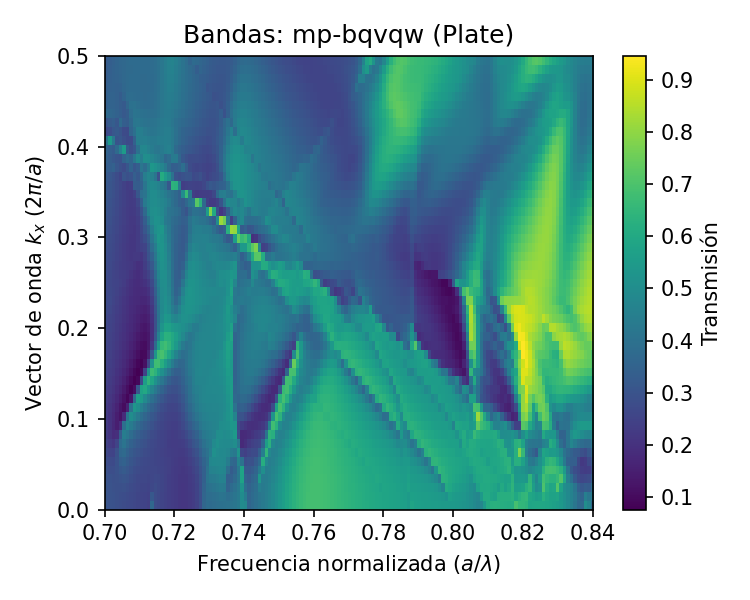
\includegraphics[width=0.48\textwidth]{figures/mp-bqvqw_plate.png}
\hfill
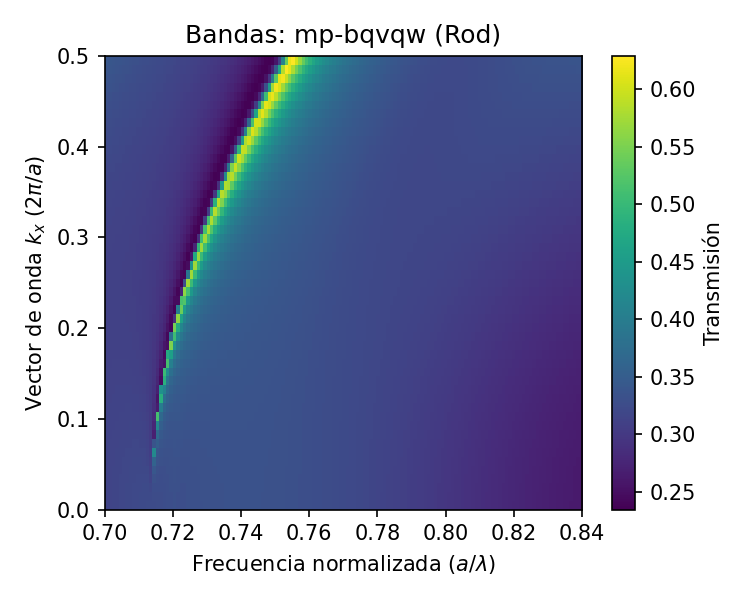
\includegraphics[width=0.48\textwidth]{figures/mp-bqvqw_rod.png}
\caption{Estructuras de bandas fotónicas ($k_x$) para mp-bqvqw. Izquierda: Lámina. Derecha: Cilindros.}
\end{figure}
\vspace{1em}
\begin{figure}[H]
\centering
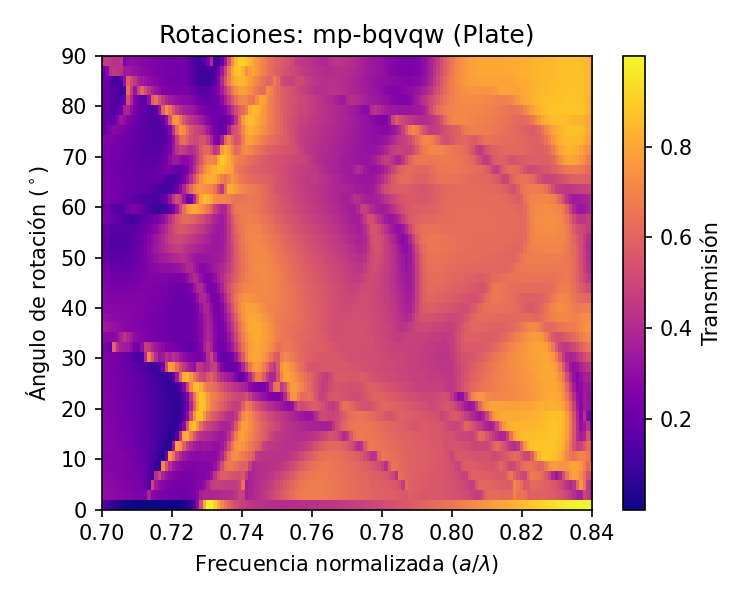
\includegraphics[width=0.48\textwidth]{figures/mp-bqvqw_plate_rangle.png}
\hfill
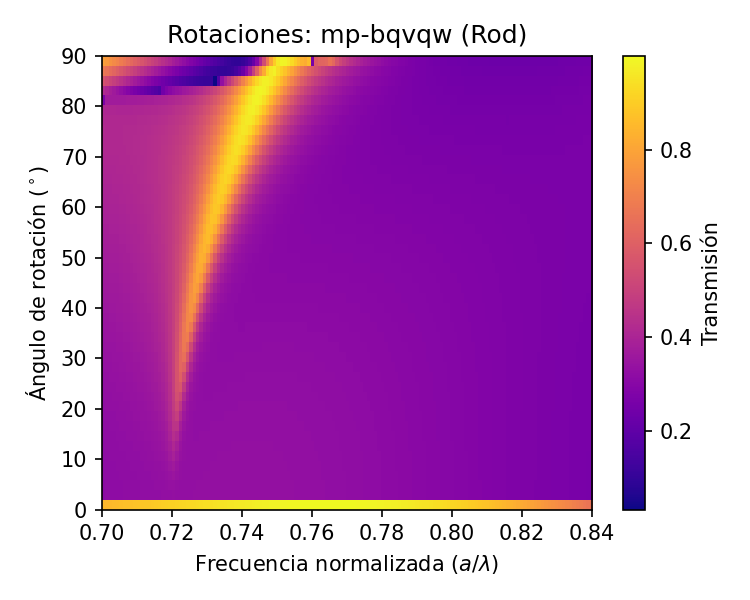
\includegraphics[width=0.48\textwidth]{figures/mp-bqvqw_rod_rangle.png}
\caption{Mapas de transmisión por rotación (twist) para mp-bqvqw. Izquierda: Lámina. Derecha: Cilindros.}
\end{figure}
\vspace{1em}
\hrule
\vspace{1em}
\subsection*{Material ID: mp-bqxzl}
\textbf{Constante Dieléctrica ($\epsilon_{total}$):} 7.76 \\[0.5em]
\begin{table}[h!]
\centering
\begin{tabular}{lcc}
\toprule
\textbf{Métrica} & \textbf{Lámina (Plate)} & \textbf{Cilindros (Rod)} \\
\midrule
Bandgaps ($k_x$) & Ninguno & Ninguno \\
Resonancias ($k_x$) & 36 & 36 \\
\midrule
Bandgaps (Rotación) & Ninguno & Ninguno \\
Resonancias (Rotación) & 33 & 33 \\
\bottomrule
\end{tabular}
\end{table}
\begin{figure}[H]
\centering
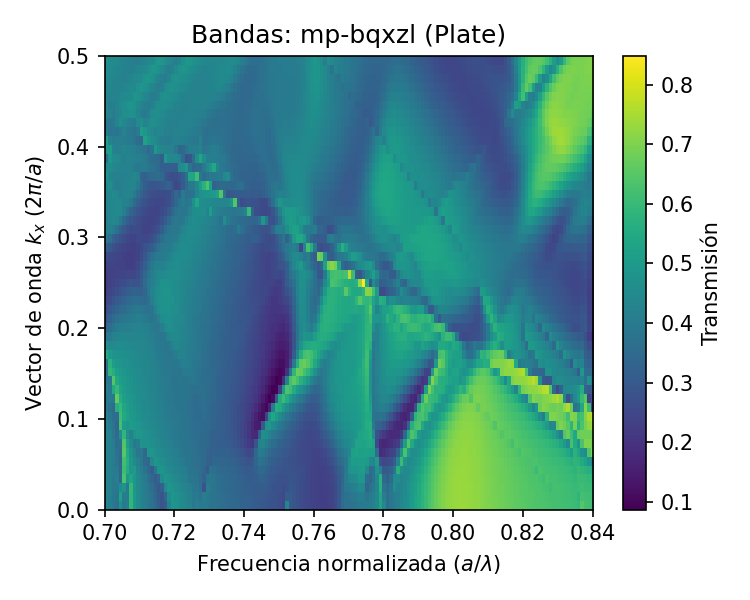
\includegraphics[width=0.48\textwidth]{figures/mp-bqxzl_plate.png}
\hfill
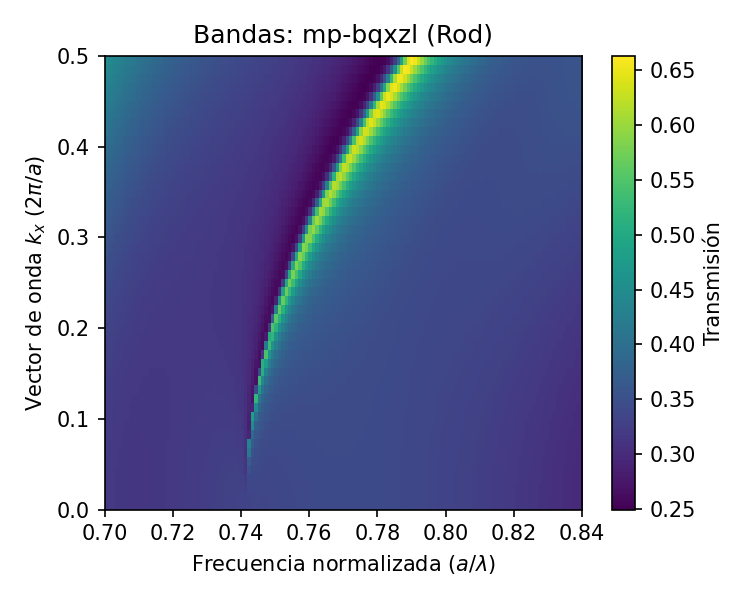
\includegraphics[width=0.48\textwidth]{figures/mp-bqxzl_rod.png}
\caption{Estructuras de bandas fotónicas ($k_x$) para mp-bqxzl. Izquierda: Lámina. Derecha: Cilindros.}
\end{figure}
\vspace{1em}
\begin{figure}[H]
\centering
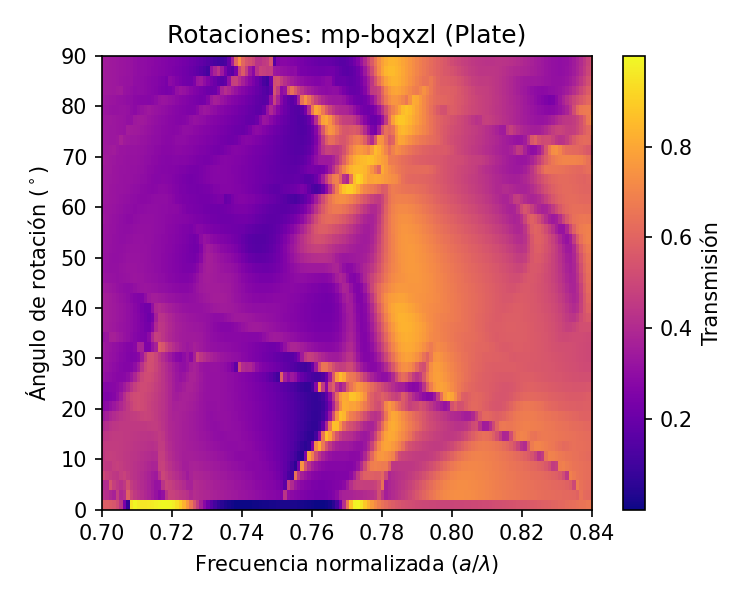
\includegraphics[width=0.48\textwidth]{figures/mp-bqxzl_plate_rangle.png}
\hfill
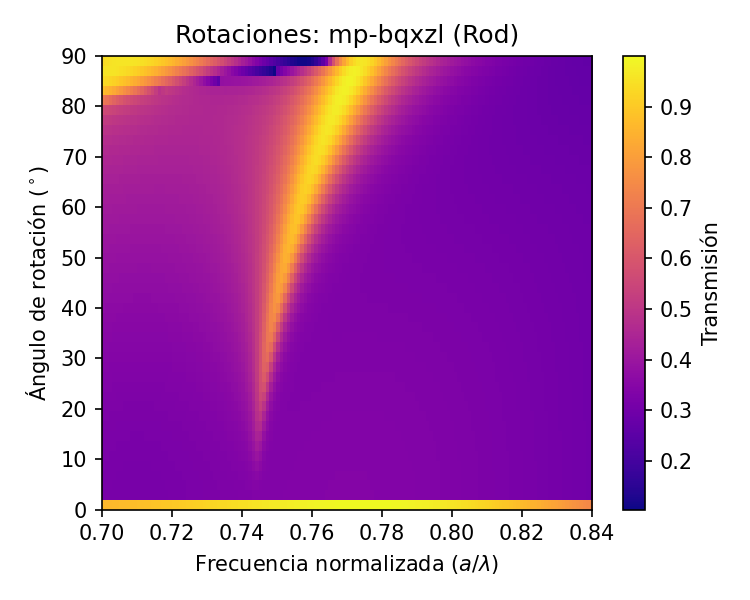
\includegraphics[width=0.48\textwidth]{figures/mp-bqxzl_rod_rangle.png}
\caption{Mapas de transmisión por rotación (twist) para mp-bqxzl. Izquierda: Lámina. Derecha: Cilindros.}
\end{figure}
\vspace{1em}
\hrule
\vspace{1em}
\subsection*{Material ID: mp-bqypg}
\textbf{Constante Dieléctrica ($\epsilon_{total}$):} 7.70 \\[0.5em]
\begin{table}[h!]
\centering
\begin{tabular}{lcc}
\toprule
\textbf{Métrica} & \textbf{Lámina (Plate)} & \textbf{Cilindros (Rod)} \\
\midrule
Bandgaps ($k_x$) & Ninguno & Ninguno \\
Resonancias ($k_x$) & 36 & 36 \\
\midrule
Bandgaps (Rotación) & Ninguno & Ninguno \\
Resonancias (Rotación) & 33 & 33 \\
\bottomrule
\end{tabular}
\end{table}
\begin{figure}[H]
\centering
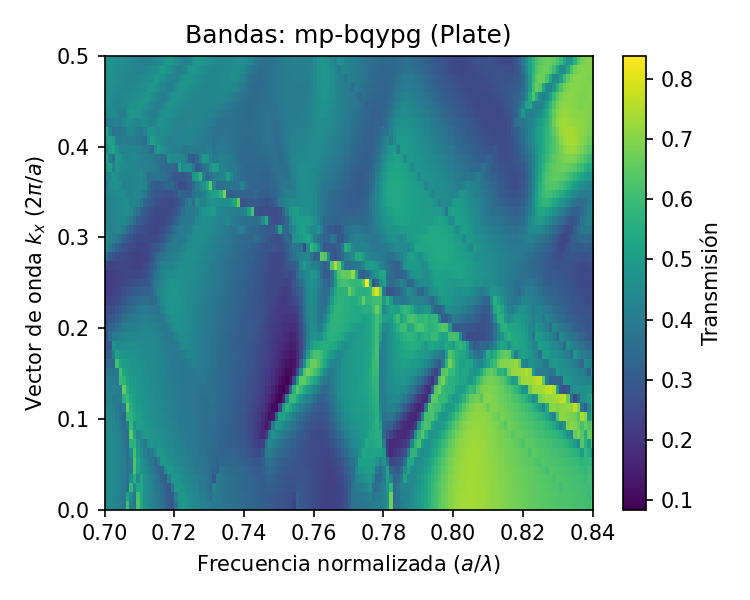
\includegraphics[width=0.48\textwidth]{figures/mp-bqypg_plate.png}
\hfill
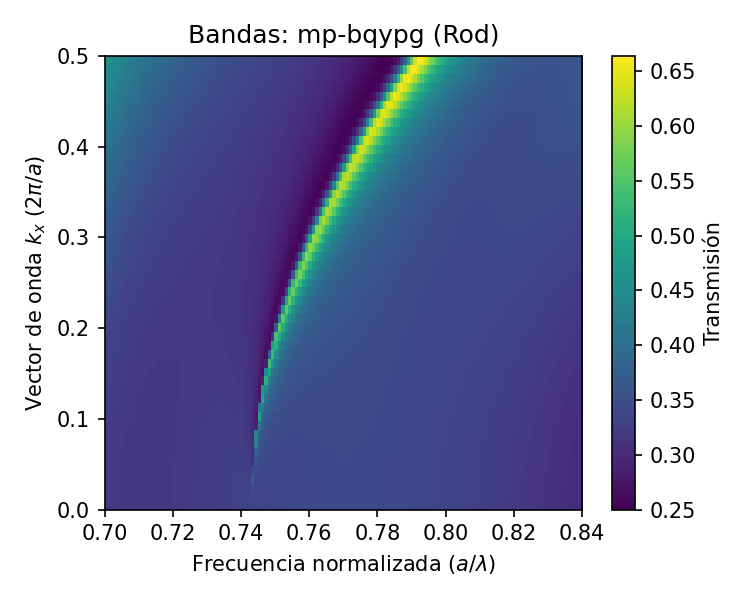
\includegraphics[width=0.48\textwidth]{figures/mp-bqypg_rod.png}
\caption{Estructuras de bandas fotónicas ($k_x$) para mp-bqypg. Izquierda: Lámina. Derecha: Cilindros.}
\end{figure}
\vspace{1em}
\begin{figure}[H]
\centering
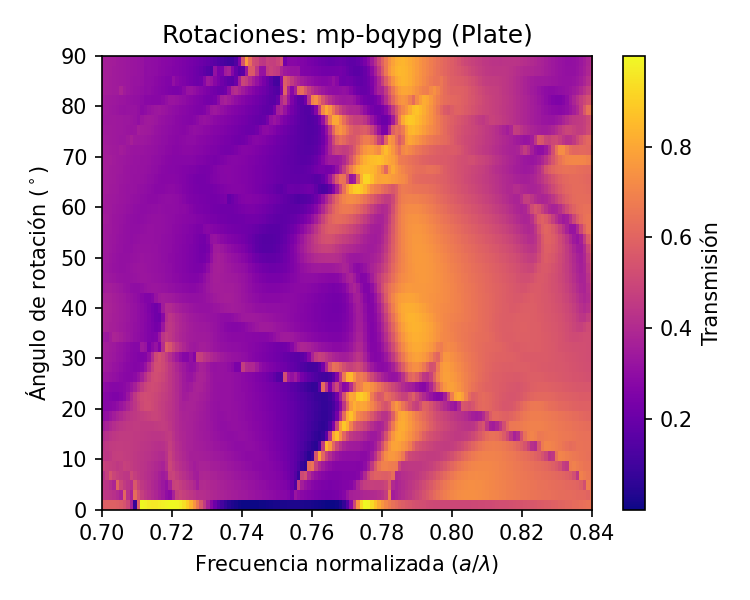
\includegraphics[width=0.48\textwidth]{figures/mp-bqypg_plate_rangle.png}
\hfill
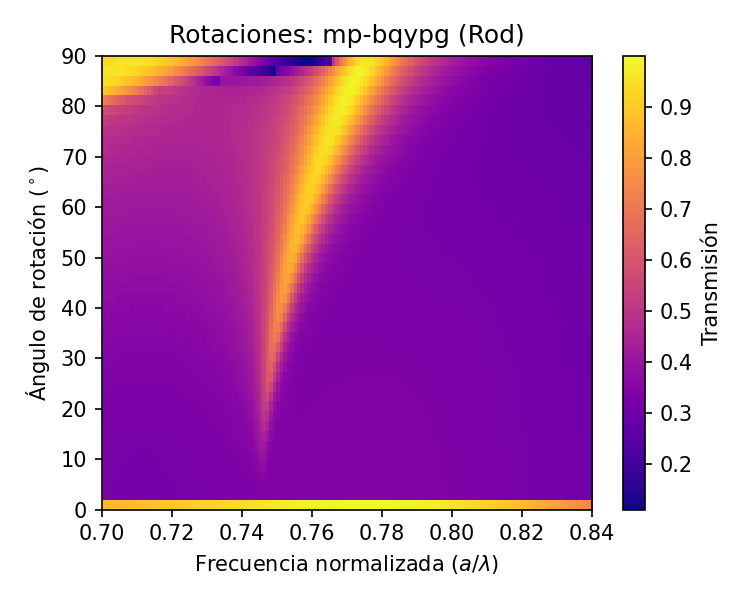
\includegraphics[width=0.48\textwidth]{figures/mp-bqypg_rod_rangle.png}
\caption{Mapas de transmisión por rotación (twist) para mp-bqypg. Izquierda: Lámina. Derecha: Cilindros.}
\end{figure}
\vspace{1em}
\hrule
\vspace{1em}
\subsection*{Material ID: mp-bqzpb}
\textbf{Constante Dieléctrica ($\epsilon_{total}$):} 13.92 \\[0.5em]
\begin{table}[h!]
\centering
\begin{tabular}{lcc}
\toprule
\textbf{Métrica} & \textbf{Lámina (Plate)} & \textbf{Cilindros (Rod)} \\
\midrule
Bandgaps ($k_x$) & Ninguno & Ninguno \\
Resonancias ($k_x$) & 36 & 36 \\
\midrule
Bandgaps (Rotación) & Ninguno & Ninguno \\
Resonancias (Rotación) & 33 & 33 \\
\bottomrule
\end{tabular}
\end{table}
\begin{figure}[H]
\centering
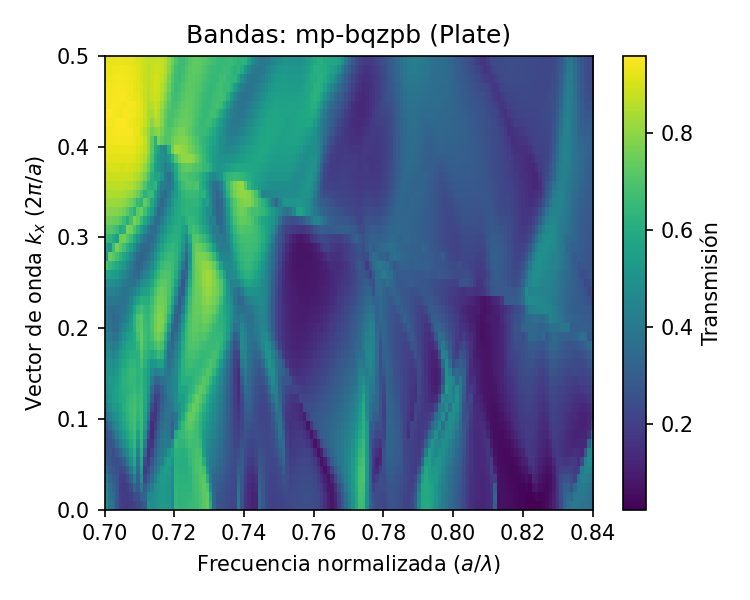
\includegraphics[width=0.48\textwidth]{figures/mp-bqzpb_plate.png}
\hfill
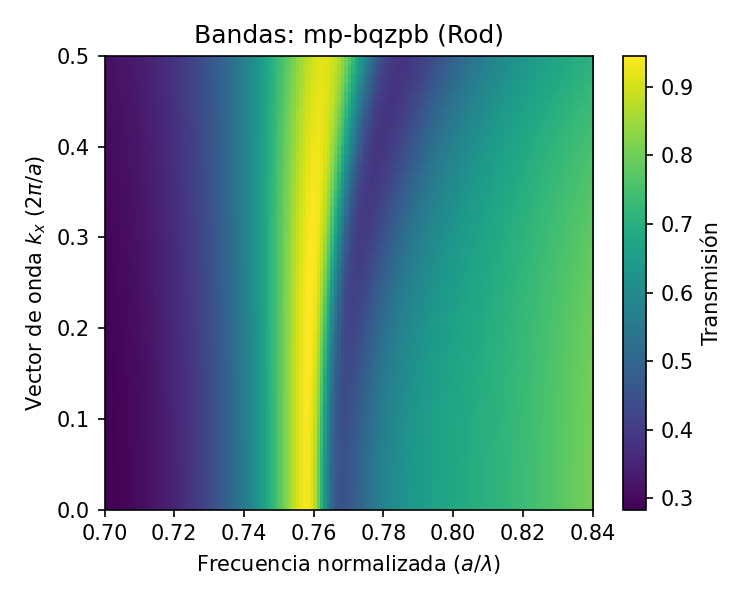
\includegraphics[width=0.48\textwidth]{figures/mp-bqzpb_rod.png}
\caption{Estructuras de bandas fotónicas ($k_x$) para mp-bqzpb. Izquierda: Lámina. Derecha: Cilindros.}
\end{figure}
\vspace{1em}
\begin{figure}[H]
\centering
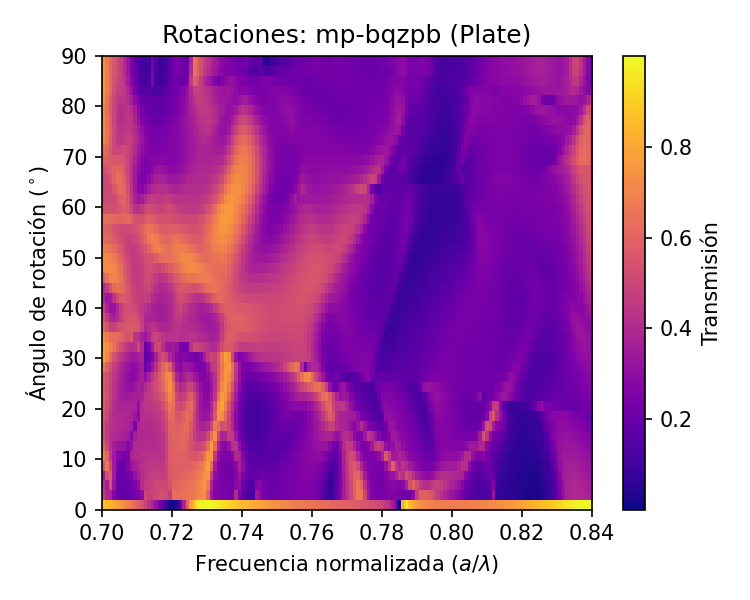
\includegraphics[width=0.48\textwidth]{figures/mp-bqzpb_plate_rangle.png}
\hfill
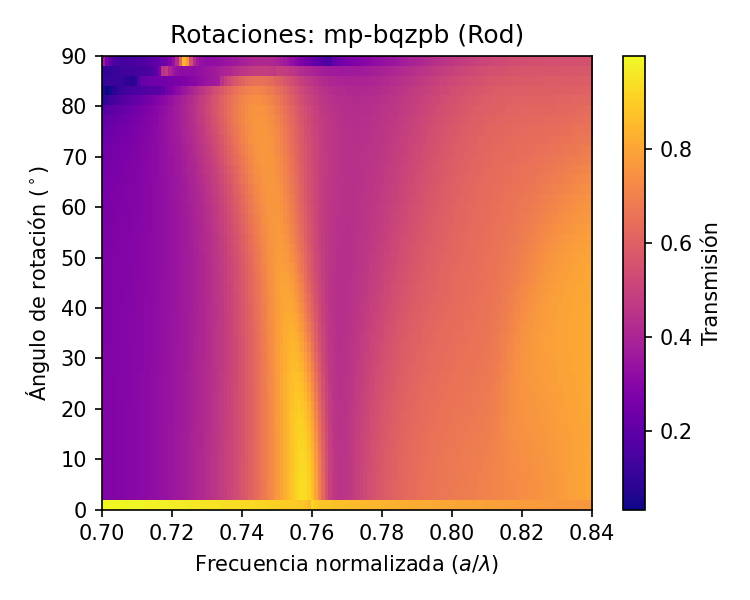
\includegraphics[width=0.48\textwidth]{figures/mp-bqzpb_rod_rangle.png}
\caption{Mapas de transmisión por rotación (twist) para mp-bqzpb. Izquierda: Lámina. Derecha: Cilindros.}
\end{figure}
\vspace{1em}
\hrule
\vspace{1em}
\subsection*{Material ID: mp-brz}
\textbf{Constante Dieléctrica ($\epsilon_{total}$):} 9.71 \\[0.5em]
\begin{table}[h!]
\centering
\begin{tabular}{lcc}
\toprule
\textbf{Métrica} & \textbf{Lámina (Plate)} & \textbf{Cilindros (Rod)} \\
\midrule
Bandgaps ($k_x$) & Ninguno & Ninguno \\
Resonancias ($k_x$) & 36 & 36 \\
\midrule
Bandgaps (Rotación) & Ninguno & Ninguno \\
Resonancias (Rotación) & 33 & 33 \\
\bottomrule
\end{tabular}
\end{table}
\begin{figure}[H]
\centering
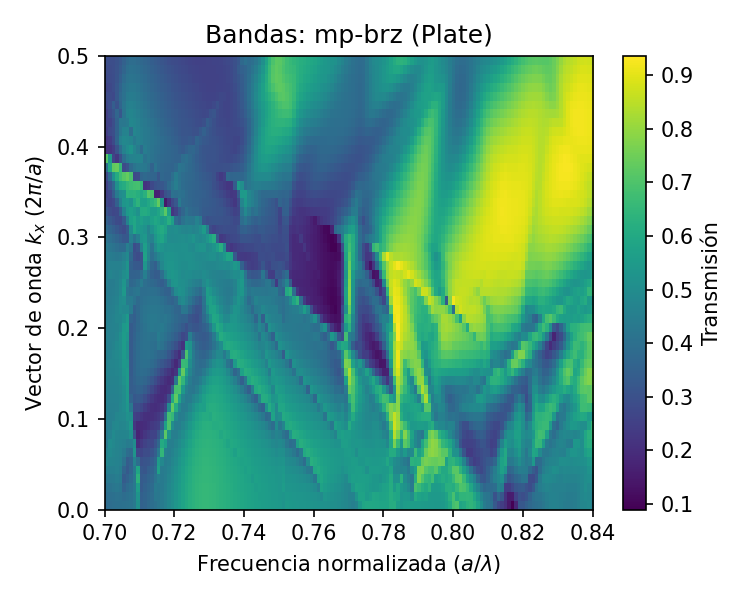
\includegraphics[width=0.48\textwidth]{figures/mp-brz_plate.png}
\hfill
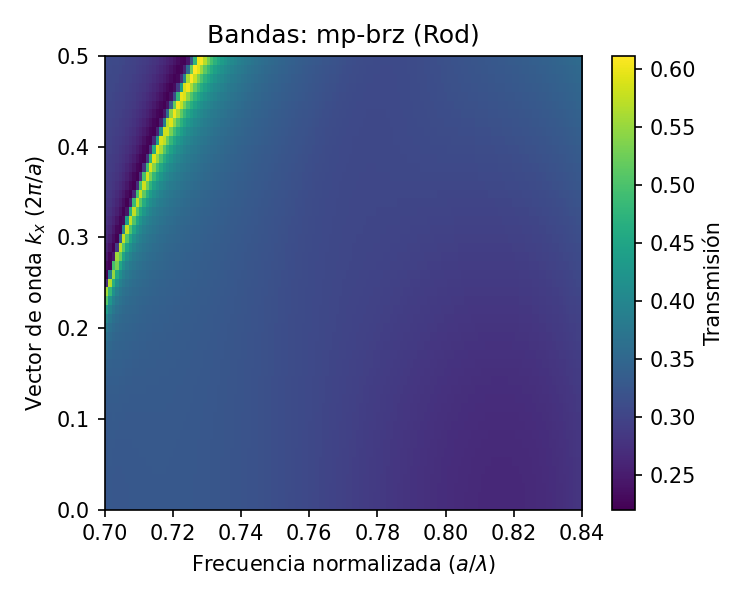
\includegraphics[width=0.48\textwidth]{figures/mp-brz_rod.png}
\caption{Estructuras de bandas fotónicas ($k_x$) para mp-brz. Izquierda: Lámina. Derecha: Cilindros.}
\end{figure}
\vspace{1em}
\begin{figure}[H]
\centering
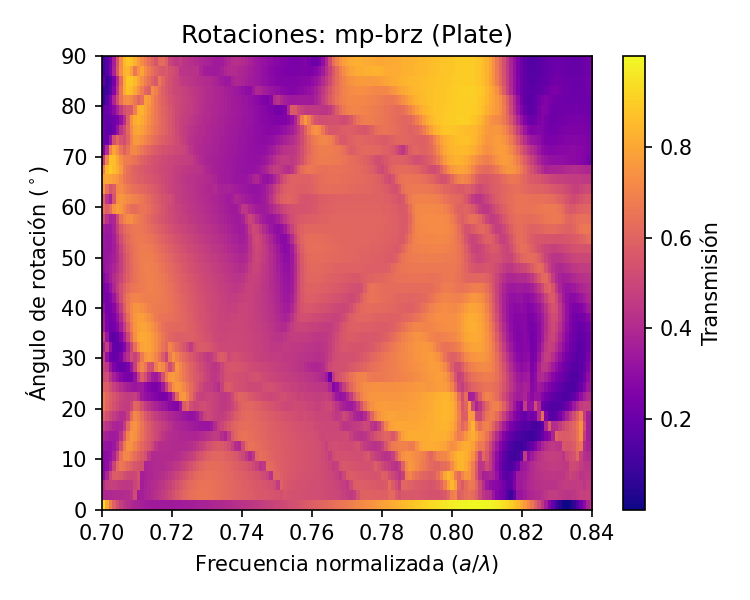
\includegraphics[width=0.48\textwidth]{figures/mp-brz_plate_rangle.png}
\hfill
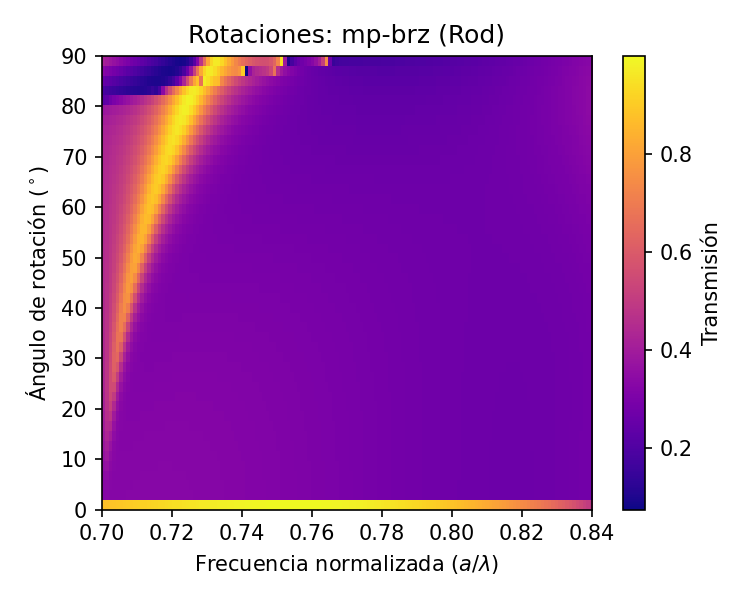
\includegraphics[width=0.48\textwidth]{figures/mp-brz_rod_rangle.png}
\caption{Mapas de transmisión por rotación (twist) para mp-brz. Izquierda: Lámina. Derecha: Cilindros.}
\end{figure}
\vspace{1em}
\hrule
\vspace{1em}
\subsection*{Material ID: mp-bwes}
\textbf{Constante Dieléctrica ($\epsilon_{total}$):} 9.08 \\[0.5em]
\begin{table}[h!]
\centering
\begin{tabular}{lcc}
\toprule
\textbf{Métrica} & \textbf{Lámina (Plate)} & \textbf{Cilindros (Rod)} \\
\midrule
Bandgaps ($k_x$) & Ninguno & Ninguno \\
Resonancias ($k_x$) & 36 & 36 \\
\midrule
Bandgaps (Rotación) & Ninguno & Ninguno \\
Resonancias (Rotación) & 33 & 33 \\
\bottomrule
\end{tabular}
\end{table}
\begin{figure}[H]
\centering
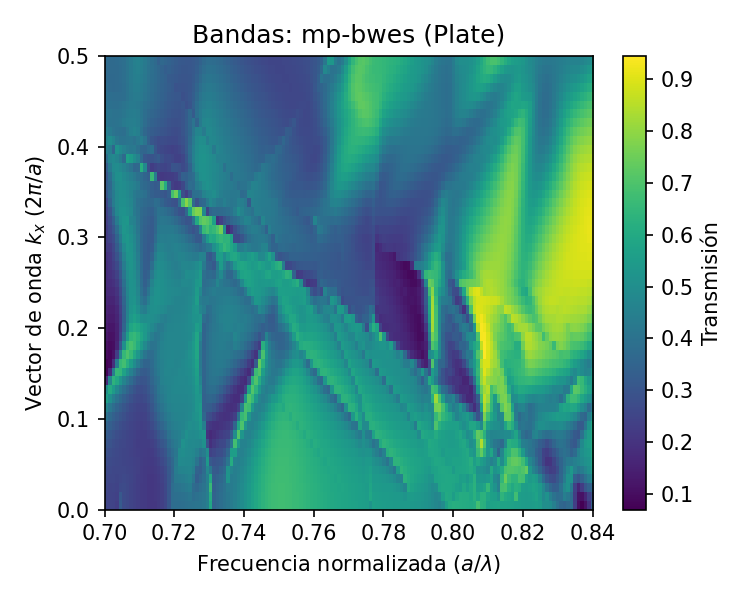
\includegraphics[width=0.48\textwidth]{figures/mp-bwes_plate.png}
\hfill
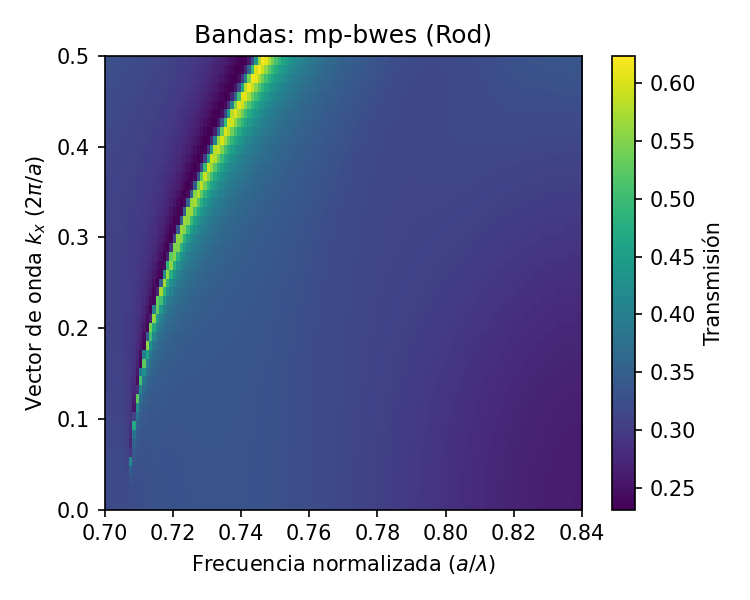
\includegraphics[width=0.48\textwidth]{figures/mp-bwes_rod.png}
\caption{Estructuras de bandas fotónicas ($k_x$) para mp-bwes. Izquierda: Lámina. Derecha: Cilindros.}
\end{figure}
\vspace{1em}
\begin{figure}[H]
\centering
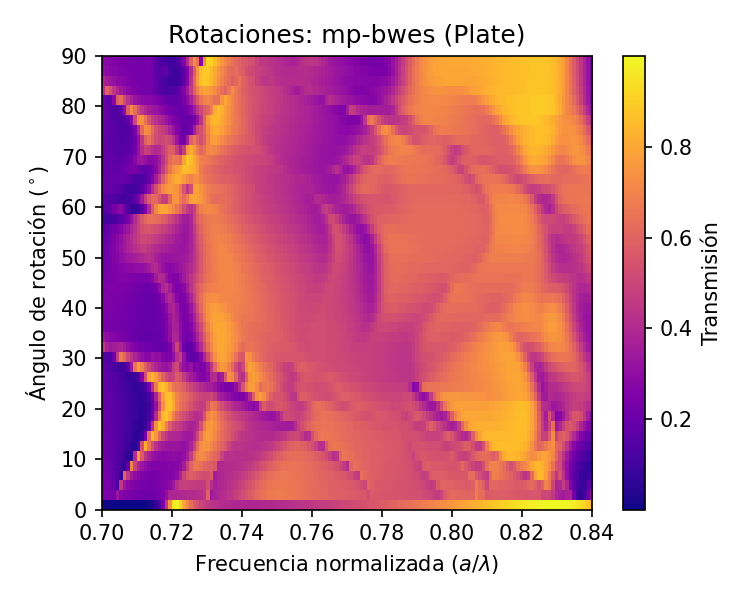
\includegraphics[width=0.48\textwidth]{figures/mp-bwes_plate_rangle.png}
\hfill
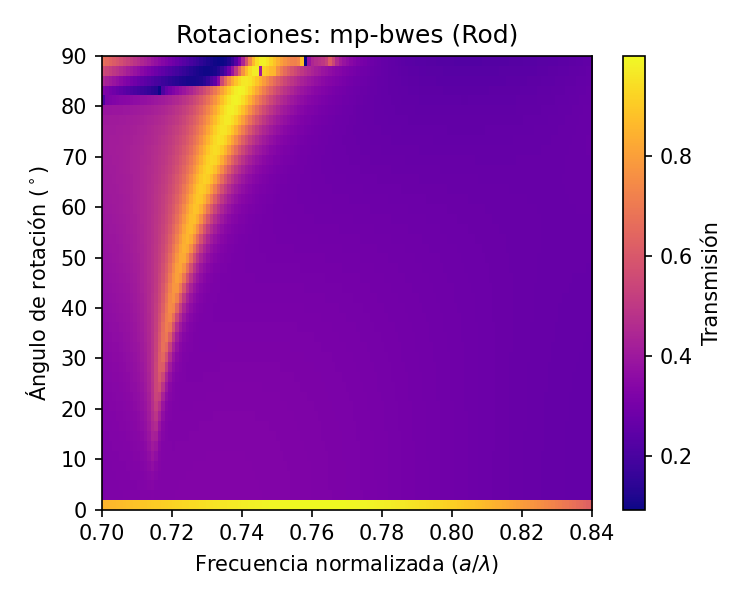
\includegraphics[width=0.48\textwidth]{figures/mp-bwes_rod_rangle.png}
\caption{Mapas de transmisión por rotación (twist) para mp-bwes. Izquierda: Lámina. Derecha: Cilindros.}
\end{figure}
\vspace{1em}
\hrule
\vspace{1em}
\subsection*{Material ID: mp-klc}
\textbf{Constante Dieléctrica ($\epsilon_{total}$):} 8.98 \\[0.5em]
\begin{table}[h!]
\centering
\begin{tabular}{lcc}
\toprule
\textbf{Métrica} & \textbf{Lámina (Plate)} & \textbf{Cilindros (Rod)} \\
\midrule
Bandgaps ($k_x$) & Ninguno & Ninguno \\
Resonancias ($k_x$) & 36 & 36 \\
\midrule
Bandgaps (Rotación) & Ninguno & Ninguno \\
Resonancias (Rotación) & 33 & 33 \\
\bottomrule
\end{tabular}
\end{table}
\begin{figure}[H]
\centering
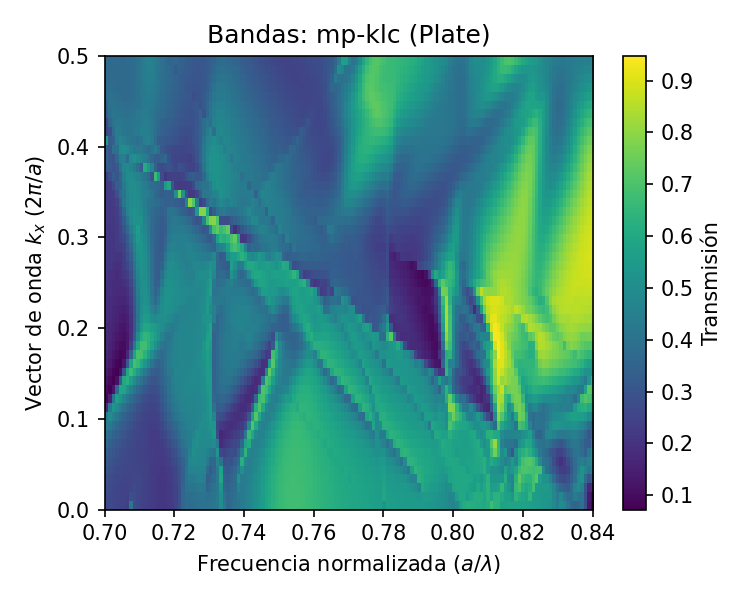
\includegraphics[width=0.48\textwidth]{figures/mp-klc_plate.png}
\hfill
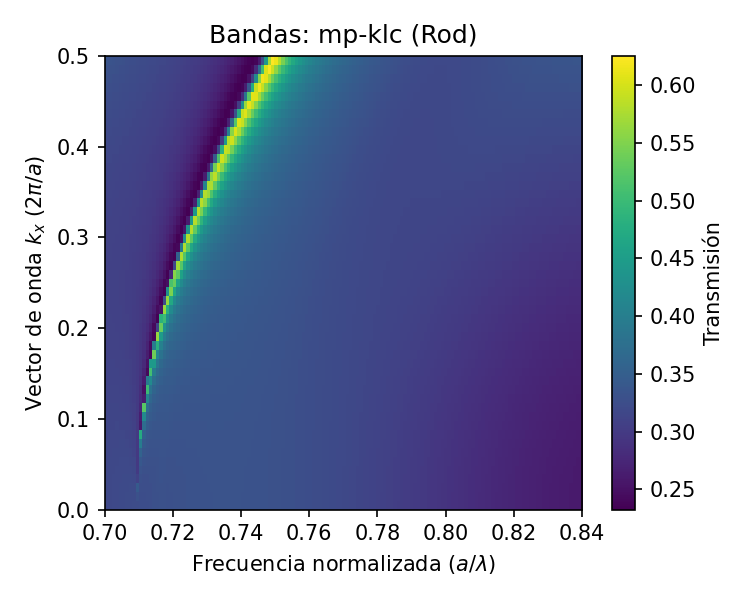
\includegraphics[width=0.48\textwidth]{figures/mp-klc_rod.png}
\caption{Estructuras de bandas fotónicas ($k_x$) para mp-klc. Izquierda: Lámina. Derecha: Cilindros.}
\end{figure}
\vspace{1em}
\begin{figure}[H]
\centering
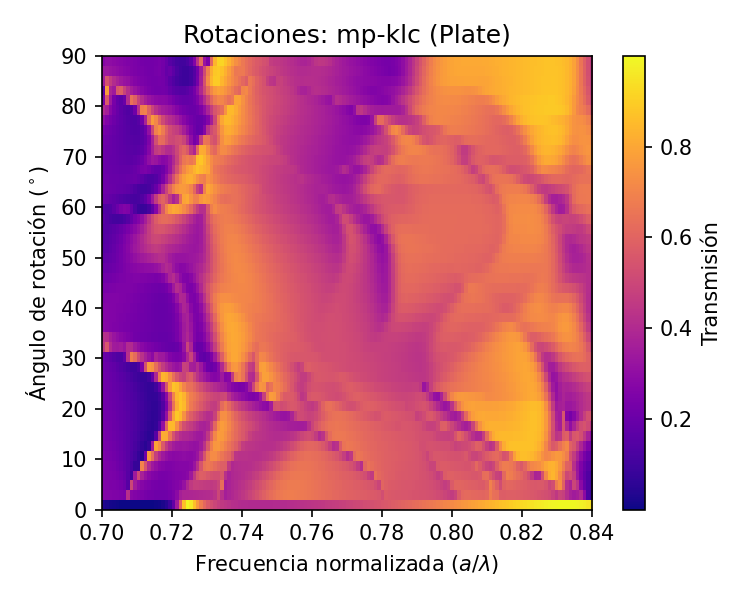
\includegraphics[width=0.48\textwidth]{figures/mp-klc_plate_rangle.png}
\hfill
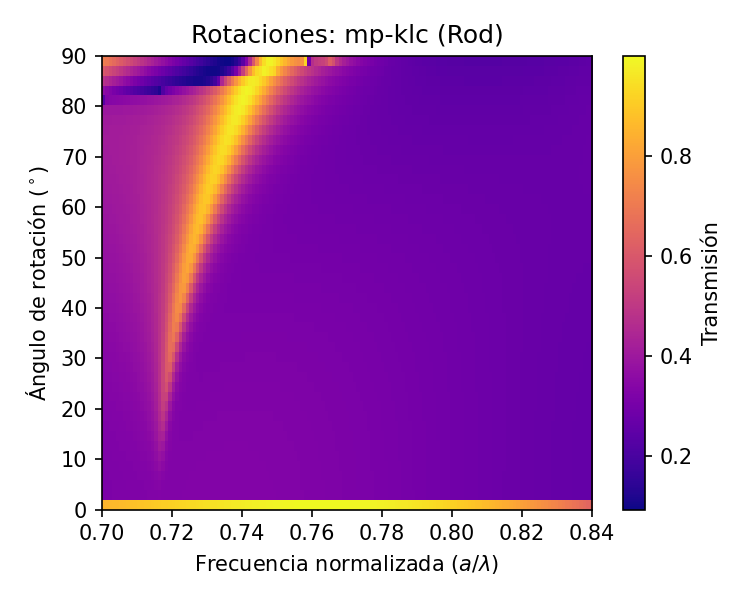
\includegraphics[width=0.48\textwidth]{figures/mp-klc_rod_rangle.png}
\caption{Mapas de transmisión por rotación (twist) para mp-klc. Izquierda: Lámina. Derecha: Cilindros.}
\end{figure}
\vspace{1em}
\hrule
\vspace{1em}
\clearpage